\documentclass{article}
\usepackage{tikz}
\usepackage{pgfplots}
\pgfplotsset{compat=1.17}
\begin{document}
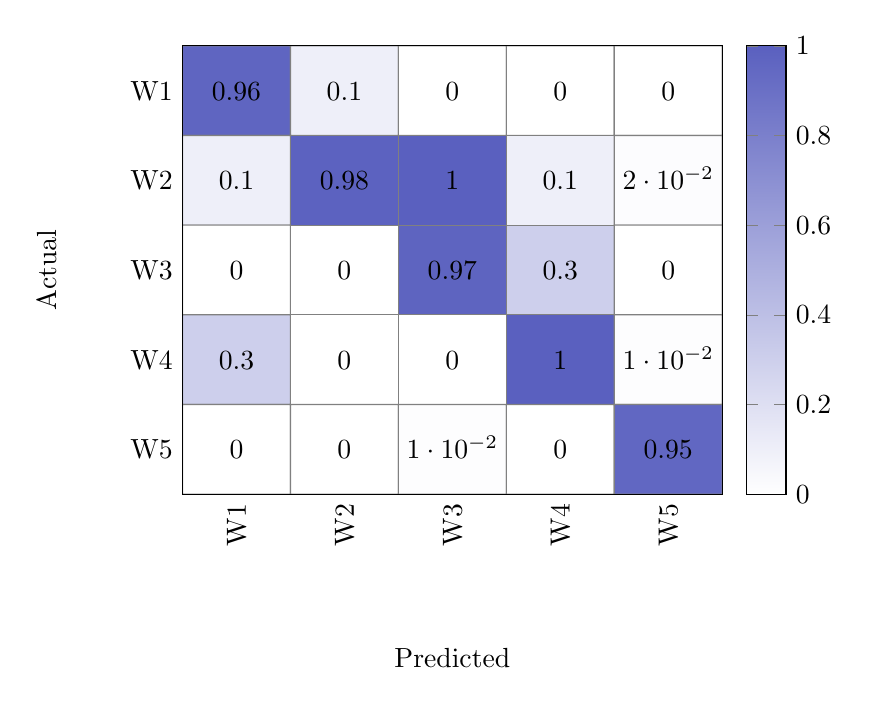
\begin{tikzpicture}
    \begin{axis}[
            colormap={bluewhite}{color=(white) rgb255=(90,96,191)},
            xlabel=Predicted,
            xlabel style={yshift=-30pt},
            ylabel=Actual,
            ylabel style={yshift=20pt},
            xticklabels={W1, W2, W3, W4, W5}, % changed
            xtick={0,...,4}, % changed
            xtick style={draw=none},
            yticklabels={W1, W2, W3, W4, W5}, % changed
            ytick={0,...,4}, % changed
            ytick style={draw=none},
            enlargelimits=false,
            colorbar,
            xticklabel style={
              rotate=90
            },
            nodes near coords={\pgfmathprintnumber\pgfplotspointmeta},
            nodes near coords style={
                yshift=-7pt
            },
        ]
        \addplot[
            matrix plot,
            mesh/cols=5, % changed
            point meta=explicit,draw=gray
        ] table [meta=C] {
            x y C
            0 0 0.96
            1 0 0.1
            2 0 0
            3 0 0
            4 0 0
            
            0 1 0.1
            1 1 0.98
            2 1 1
            3 1 0.1
            4 1 0.02
            
            0 2 0
            1 2 0
            2 2 0.97
            3 2 0.3
            4 2 0
    
            0 3 0.3
            1 3 0
            2 3 0
            3 3 1
            4 3 0.01
    
            0 4 0
            1 4 0
            2 4 0.01
            3 4 0
            4 4 0.95
            
        }; % added every entry where x=4 or y=4
    \end{axis}
\end{tikzpicture}
\end{document}